%\RequirePackage[l2tabu, orthodox]{nag}
\RequirePackage{currfile}
\documentclass[12pt]{beamer}
\graphicspath{{Imagenes/}{../Imagenes/}}
\usepackage[utf8]{inputenc}
\usepackage[spanish]{babel}
\usepackage{standalone}
\usepackage{color}
\usepackage[binary-units=true]{siunitx}
\usepackage{hyperref}
\hypersetup{
  colorlinks=true,
  linkcolor=blue,          % color of internal links (change box color with linkbordercolor)
  citecolor=green,        % color of links to bibliography
  filecolor=magenta,      % color of file links
  urlcolor=cyan,           % color of external links
  linkbordercolor={0 0 1}
}
\usepackage{xcolor, soul}
\usepackage{etoolbox}
\usepackage{amsmath}
\usepackage{amsthm}
\usepackage{physics}
\usepackage{multicol}
\usepackage{graphicx}
\usepackage{bookmark}
\usepackage{longtable}
\usepackage{graphicx}
\usepackage{tikz}
\usepackage[siunitx, RPvoltages]{circuitikz}
\usetikzlibrary{mindmap}
\usetikzlibrary{arrows, patterns, shapes, decorations.markings, decorations.pathmorphing}
\usetikzlibrary{matrix,positioning}
\tikzstyle{every picture}+=[remember picture,baseline]
\usepackage[autostyle,spanish=mexican]{csquotes}
\usepackage{pifont}
\usepackage[font=footnotesize,textfont=it]{caption}
\usepackage{tabulary}
\usepackage{booktabs}
\usepackage[outdir=./]{epstopdf}
%\usepackage{epstopdf}
\usepackage{media9}
\usepackage{multimedia}
\usepackage{bigints}
%\usepackage{enumitem}
\usepackage[os=win]{menukeys}
\usepackage{pifont}
\usepackage{pbox}
\usepackage{alltt}
\usepackage{verbatim}
\usepackage{colortbl}
\usepackage{tcolorbox}
\usepackage{fancyvrb}
\usepackage[sfdefault]{roboto}  %% Option 'sfdefault' only if the base font of the document is to be sans serif
%\usepackage[T1]{fontenc}
\setcounter{secnumdepth}{3}
\setcounter{tocdepth}{3}
\DeclareGraphicsExtensions{.pdf,.png,.jpg}
\renewcommand {\arraystretch}{1.5}
\definecolor{ao}{rgb}{0.0, 0.5, 0.0}
\definecolor{aquamarine}{rgb}{0.5, 1.0, 0.83}
\definecolor{kellygreen}{rgb}{0.3, 0.73, 0.09}
\definecolor{bisque}{rgb}{1.0, 0.89, 0.77}
\definecolor{amber}{rgb}{1.0, 0.75, 0.0}
\definecolor{armygreen}{rgb}{0.29, 0.33, 0.13}
\definecolor{alizarin}{rgb}{0.82, 0.1, 0.26}
\definecolor{cadetblue}{rgb}{0.37, 0.62, 0.63}
\newcommand*{\TitleParbox}[1]{\parbox[c]{6cm}{\raggedright #1}}%
\newcommand{\python}{\texttt{python}}
\newcommand{\textoazul}[1]{\textcolor{blue}{#1}}
\newcommand{\azulfuerte}[1]{\textcolor{blue}{\textbf{#1}}}
\newcommand{\funcionazul}[1]{\textcolor{blue}{\textbf{\texttt{#1}}}}
%\normalfont
\usepackage{ccfonts}% http://ctan.org/pkg/{ccfonts}
\usepackage[T1]{fontenc}% http://ctan.or/pkg/fontenc
\renewcommand{\rmdefault}{cmr}% cmr = Computer Modern Roman
\usefonttheme[onlymath]{serif}
\linespread{1.3}
\newcounter{saveenumi}
\newcommand{\seti}{\setcounter{saveenumi}{\value{enumi}}}
\newcommand{\conti}{\setcounter{enumi}{\value{saveenumi}}}
\newcommand{\tikzmark}[1]{\tikz[remember picture] \node[coordinate] (#1) {#1};}

\usepackage{scalerel}[2016-12-29]
\def\stretchint#1{\vcenter{\hbox{\stretchto[440]{\displaystyle\int}{#1}}}}
\def\scaleint#1{\vcenter{\hbox{\scaleto[3ex]{\displaystyle\int}{#1}}}}
\def\bs{\mkern-12mu}

\newtheorem{teo}{}[section]
\usepackage{blkarray}

%reduce el tamaño de letra de la etiqueta equations
\makeatletter
\def\maketag@@@#1{\hbox{\m@th\normalfont\small#1}}
\makeatother

%se usa para la x en itemize
\newcommand{\xmark}{\text{\ding{55}}}

%\AtBeginDocument{\setlength{\tymin}{1em}}


\definecolor{myblue}{rgb}{.8, .8, 1}

\usepackage{empheq}

\newlength\mytemplen
\newsavebox\mytempbox

\makeatletter
\newcommand\mybluebox{%
    \@ifnextchar[%]
       {\@mybluebox}%
       {\@mybluebox[0pt]}}

\def\@mybluebox[#1]{%
    \@ifnextchar[%]
       {\@@mybluebox[#1]}%
       {\@@mybluebox[#1][0pt]}}

\def\@@mybluebox[#1][#2]#3{
    \sbox\mytempbox{#3}%
    \mytemplen\ht\mytempbox
    \advance\mytemplen #1\relax
    \ht\mytempbox\mytemplen
    \mytemplen\dp\mytempbox
    \advance\mytemplen #2\relax
    \dp\mytempbox\mytemplen
    \colorbox{myblue}{\hspace{1em}\usebox{\mytempbox}\hspace{1em}}}

\makeatother



%Se usa la plantilla Madrid modificada con beaver
\mode<presentation>
{
  \usetheme{Madrid}
  \setbeamertemplate{headline}{}
  %\useoutertheme{infolines}
  \usecolortheme{beaver}
  \setbeamercovered{invisible}
  

\setbeamertemplate{section in toc}[sections numbered]
\setbeamertemplate{subsection in toc}[subsections numbered]
\setbeamertemplate{subsection in toc}{\leavevmode\leftskip=3.2em\rlap{\hskip-2em\inserttocsectionnumber.\inserttocsubsectionnumber}\inserttocsubsection\par}
\setbeamercolor{section in toc}{fg=blue}
\setbeamercolor{subsection in toc}{fg=blue}
\setbeamerfont{subsection in toc}{size=\small}

\setbeamertemplate{navigation symbols}{}
\setbeamertemplate{caption}[numbered]

}

\usepackage{courier}
\usepackage{listingsutf8}
\usepackage{listings}
\usepackage{xcolor}
\usepackage{textcomp}
\usepackage{color}
\definecolor{deepblue}{rgb}{0,0,0.5}
\definecolor{brown}{rgb}{0.59, 0.29, 0.0}
\definecolor{OliveGreen}{rgb}{0,0.25,0}
% \usepackage{minted}

\DeclareCaptionFont{white}{\color{white}}
\DeclareCaptionFormat{listing}{\colorbox{gray}{\parbox{0.98\textwidth}{#1#2#3}}}
\captionsetup[lstlisting]{format=listing,labelfont=white,textfont=white}
\renewcommand{\lstlistingname}{Código}


\definecolor{Code}{rgb}{0,0,0}
\definecolor{Keywords}{rgb}{255,0,0}
\definecolor{Strings}{rgb}{255,0,255}
\definecolor{Comments}{rgb}{0,0,255}
\definecolor{Numbers}{rgb}{255,128,0}

\makeatletter

\newif\iffirstchar\firstchartrue
\newif\ifstartedbyadigit
\newif\ifprecededbyequalsign

\newcommand\processletter
{%
  \ifnum\lst@mode=\lst@Pmode%
    \iffirstchar%
        \global\startedbyadigitfalse%
      \fi
      \global\firstcharfalse%
    \fi
}

\newcommand\processdigit
{%
  \ifnum\lst@mode=\lst@Pmode%
      \iffirstchar%
        \global\startedbyadigittrue%
      \fi
      \global\firstcharfalse%
  \fi
}

\lst@AddToHook{OutputOther}%
{%
  \lst@IfLastOtherOneOf{=}
    {\global\precededbyequalsigntrue}
    {}%
}

\lst@AddToHook{Output}%
{%
  \ifprecededbyequalsign%
      \ifstartedbyadigit%
        \def\lst@thestyle{\color{orange}}%
      \fi
    \fi
  \global\firstchartrue%
  \global\startedbyadigitfalse%
  \global\precededbyequalsignfalse%
}

\lstset{ 
language=Python,                % choose the language of the code
basicstyle=\footnotesize\ttfamily,       % the size of the fonts that are used for the code
numbers=left,                   % where to put the line-numbers
numberstyle=\scriptsize,      % the size of the fonts that are used for the line-numbers
stepnumber=1,                   % the step between two line-numbers. If it is 1 each line will be numbered
numbersep=5pt,                  % how far the line-numbers are from the code
backgroundcolor=\color{white},  % choose the background color. You must add \usepackage{color}
showspaces=false,               % show spaces adding particular underscores
showstringspaces=false,         % underline spaces within strings
showtabs=false,                 % show tabs within strings adding particular underscores
frame=single,   		% adds a frame around the code
tabsize=2,  		% sets default tabsize to 2 spaces
captionpos=t,   		% sets the caption-position to bottom
breaklines=true,    	% sets automatic line breaking
breakatwhitespace=false,    % sets if automatic breaks should only happen at whitespace
escapeinside={\#},  % if you want to add a comment within your code
stringstyle =\color{OliveGreen},
%otherkeywords={{as}},             % Add keywords here
keywordstyle = \color{blue},
commentstyle = \color{black},
identifierstyle = \color{black},
literate=%
         {á}{{\'a}}1
         {é}{{\'e}}1
         {í}{{\'i}}1
         {ó}{{\'o}}1
         {ú}{{\'u}}1
%
%keywordstyle=\ttb\color{deepblue}
%fancyvrb = true,
}

\lstdefinestyle{FormattedNumber}{%
    literate={0}{{\textcolor{red}{0}}}{1}%
             {1}{{\textcolor{red}{1}}}{1}%
             {2}{{\textcolor{red}{2}}}{1}%
             {3}{{\textcolor{red}{3}}}{1}%
             {4}{{\textcolor{red}{4}}}{1}%
             {5}{{\textcolor{red}{5}}}{1}%
             {6}{{\textcolor{red}{6}}}{1}%
             {7}{{\textcolor{red}{7}}}{1}%
             {8}{{\textcolor{red}{8}}}{1}%
             {9}{{\textcolor{red}{9}}}{1}%
             {.0}{{\textcolor{red}{.0}}}{2}% Following is to ensure that only periods
             {.1}{{\textcolor{red}{.1}}}{2}% followed by a digit are changed.
             {.2}{{\textcolor{red}{.2}}}{2}%
             {.3}{{\textcolor{red}{.3}}}{2}%
             {.4}{{\textcolor{red}{.4}}}{2}%
             {.5}{{\textcolor{red}{.5}}}{2}%
             {.6}{{\textcolor{red}{.6}}}{2}%
             {.7}{{\textcolor{red}{.7}}}{2}%
             {.8}{{\textcolor{red}{.8}}}{2}%
             {.9}{{\textcolor{red}{.9}}}{2}%
             {\ }{{ }}{1}% handle the space
         ,%
          %mathescape=true
          escapeinside={__}
          }



\makeatletter
\setbeamercolor{section in foot}{bg=green!30!cyan, fg=black!90!orange}
\setbeamercolor{subsection in foot}{bg=red!30!cyan, fg=red}
%\setbeamercolor{date in foot}{bg=orange!30!cyan, fg=red}
\setbeamertemplate{footline}
{
  \leavevmode%
  \hbox{%
  \begin{beamercolorbox}[wd=.333333\paperwidth,ht=2.25ex,dp=1ex,center]{section in foot}%
    \usebeamerfont{section in foot} \insertsection
  \end{beamercolorbox}}%
  \begin{beamercolorbox}[wd=.333333\paperwidth,ht=2.25ex,dp=1ex,center]{subsection in foot}%
    \usebeamerfont{subsection in foot}  \insertsubsection
  \end{beamercolorbox}%
  \begin{beamercolorbox}[wd=.333333\paperwidth,ht=2.25ex,dp=1ex,right]{date in head/foot}%
    \usebeamerfont{date in head/foot} \insertshortdate{} \hspace*{2em}
    \insertframenumber{} / \inserttotalframenumber \hspace*{2ex} 
  \end{beamercolorbox}}%
  \vskip0pt%
\makeatother
\title{Cuadraturas Gaussianas}
\subtitle{Tema 2 - Operaciones matemáticas básicas}
\author{M. en C. Gustavo Contreras Mayén}
\date{\today}
\institute{Facultad de Ciencias - UNAM}
\titlegraphic{
\includegraphics[width=1.75cm]{Imagenes/escudo-facultad-ciencias}\hspace*{4.75cm}~%
   
\includegraphics[width=1.75cm]{Imagenes/escudo-unam}
}
\newtheorem{miteorema}{Teorema}
\begin{document}
\maketitle
\fontsize{14}{14}\selectfont
\spanishdecimal{.}
\setbeamercolor{frametitle}{bg=blue!30!white}
\section*{Contenido}
\frame{\tableofcontents[currentsection, hideallsubsections]}
\section{Introducción}
\frame{\tableofcontents[currentsection, hideothersubsections]}
\subsection{Segunda parte de las cuadraturas}
\begin{frame}
\frametitle{Introducción}
Las fórmulas de Newton-Cotes implican, según la construcción, que los puntos de integración \emph{estén  igualmente espaciados}.
\\
\bigskip
Para un orden dado de la fórmula, los puntos $x_{i}$ y los pesos se seguirán directamente del polinomio de interpolación de Lagrange basado en los $n$ puntos de integración.
\end{frame}
\begin{frame}
\frametitle{Introducción}
En comparación, la idea básica de las llamadas \textoazul{cuadraturas gaussianas} consiste en \emph{elegir de manera óptima tanto los puntos (abscisas) como los pesos}, para lograr la máxima precisión para ciertas clases de integrandos (por ejemplo, polinomios).
interpolación de Lagrange basado en los $n$ puntos de integración.
\end{frame}
\begin{frame}
\frametitle{Introducción}
Al disponer de un número doble de parámetros ajustables (por separado, abscisas y pesos), se pueden construir, en principio, fórmulas de cuadratura de doble orden en comparación con las fórmulas de Newton-Cotes con el mismo número de puntos de integración.
\end{frame}
\section{Cuadraturas Gaussianas}
\frame{\tableofcontents[currentsection, hideothersubsections]}
\subsection{Definición de cuadraturas}
\begin{frame}
\frametitle{Cuadraturas Gaussianas}
Hemos visto que las fórmulas de Newton-Cotes para aproximar la intregral
\begin{align*}
\int_{a}^{b} f(x) \dd{x}
\end{align*}
trabajan muy bien si $f(x)$ es una función suave, como los polinomios.
\end{frame}
\begin{frame}
\frametitle{Cuadraturas Gaussianas}
También aplica para las cuadraturas Gaussianas, ya que son buenas para estimar integrales de la forma:
\begin{align*}
\int_{a}^{b} w(x) \, f(x) \dd{x}
\end{align*}
donde $w(x)$ se denomina \emph{función de peso} que puede contener singularidades, siempre y cuando sean integrables.
\end{frame}
\begin{frame}
\frametitle{Cuadraturas Gaussianas}
Un ejemplo de este tipo, sería la integral:
\begin{align*}
\int_{0}^{1} \left(1 + x^{2} \right) \, \ln x  \dd{x}
\end{align*}
\\
\bigskip
\pause
o cuando tenemos límites de integración infinitos
\begin{align*}
\int_{0}^{\infty} \exp(-x) \, \sin x \dd{x}
\end{align*}
éstos se pueden reacomodar para calcular la integral.
\end{frame}
\begin{frame}
\frametitle{Fórmulas de integración Gaussianas}
Las fórmulas de integración Gaussianas tiene la misma forma de las reglas de Newton-Cotes:
\begin{align*}
I = \sum_{i=0}^{n} A_{i} \, f(x_{i})
\end{align*}
donde $I$ representa la aproximación al valor de la integral, la diferencia radica en la forma en que se determinan los pesos $A_{i}$ y abscisas nodales $x_{i}$.
\end{frame}
\begin{frame}
\frametitle{Fórmulas de integración Gaussianas}
En la integración de Newton-Cotes los nodos se espacian uniformemente en $(a, b)$, es decir, estaban ya predeterminadas sus ubicaciones.
\\
\bigskip
En la cuadratura de Gauss, se eligen los nodos y los pesos de modo que con la ecuación para $I$, se obtiene la integral exacta si $f(x)$ es un polinomio de grado $2 \, n + 1$ o menor, es decir:
\end{frame}
\begin{frame}
\frametitle{Cuadratura Gaussiana}
\begin{align*}
\int_{a}^{b} w(x) \, P_{m}(x) \dd{x} = \sum_{i=0}^{n} A_{i} \, P_{m}(x_{i}), \hspace{1cm} m \leq 2 \, n + 1
\end{align*}
\pause
Una manera de determinar los pesos y las abscisas es sustituir 
\begin{align*}
P_{0}(x) &= 1 \\
P_{1}(x) &= x \\
\vdots \\
P_{2 \, n + 1}(x) &= x^{2 \, n + 1}
\end{align*}
\end{frame}
\begin{frame}
\frametitle{Cuadratura Gaussiana}
Es sustituir en la ecuación anterior y resolver el sistema de $2 \, n + 2$ ecuaciones:
\begin{align*}
\int_{a}^{b} w(x) \, x^{j} \dd{x} = \sum_{i=0}^{n} A_{i} \, x_{i}^{j}, \hspace{0.6cm} j = 0, 1, \ldots, 2 \, n + 1
\end{align*}
para las incógnitas $A_{i}$ y $x_{i}$.
\end{frame}
\begin{frame}
\frametitle{Ejemplo de una cuadratura Gaussiana}
Como ejemplo veamos: sea la función de peso $w(x)$, los intervalos de integración $a$, $b$ y $n$, tal que:
\begin{align*}
w(x)= \exp(-x) \hspace{0.5cm} a = 0, b = \infty, \hspace{0.3cm} n = 1
\end{align*}
\end{frame}
\begin{frame}[fragile]
\frametitle{Ejemplo de una cuadratura Gaussiana}
Las cuatro ecuaciones que determinan $x_{0}$, $x_{1}$, $A_{0}$ y $A_{1}$ son:
\begin{align*}
\int_{0}^{\infty} \exp(-x) \dd{x} &= A_{0} + A_{1} \\[0.5em]
\visible<2->{\int_{0}^{\infty} \exp(-x) \, x \dd{x} &= A_{0} \, x_{0} + A_{1} \, x_{1}} \\[0.5em]
\visible<3->{\int_{0}^{\infty} \exp(-x) \, x^{2} \dd{x} &= A_{0} \, x_{0}^{2}+ A_{1} \, x_{1}^{2}} \\[0.5em]
\visible<4->{\int_{0}^{\infty} \exp(-x) \, x^{3} \dd{x} &= A_{0} \, x_{0}^{3} + A_{1} \, x_{1}^{3}}
\end{align*}
\end{frame}
\begin{frame}
\frametitle{Ejemplo de una cuadratura Gaussiana}
Evaluando las integrales, obtenemos
\begin{align*}
A_{0} + A_{1} &= 1 \\[0.5em]
A_{0} x_{0} + A_{1} x_{1} &= 1 \\[0.5em]
A_{0} x_{0}^{2} + A_{1} x_{1}^{2} &= 2 \\[0.5em]
A_{0} x_{0}^{3} + A_{1} x_{1}^{3} &= 6
\end{align*}
\end{frame}
\begin{frame}
\frametitle{Ejemplo de una cuadratura Gaussiana}
Cuya solución es:
\begin{align*}
x_{0} &= 2 - \sqrt{2} \hspace{0.75cm} A_{0} = \dfrac{\sqrt{2} + 1}{2 \, \sqrt{2}} \\[0.5em]
x_{1} &= 2 + \sqrt{2} \hspace{0.75cm} A_{1} = \dfrac{\sqrt{2} - 1}{2 \, \sqrt{2}}
\end{align*}
\end{frame}
\begin{frame}
\frametitle{Ejemplo de una cuadratura Gaussiana}
Por tanto la fórmula de integración obtenida es:
\begin{align*}
\int_{0}^{\infty} \exp(-x) \, f(x) \dd{x} & \simeq \dfrac{1}{2 \, \sqrt{2}} \left[ \left( \sqrt{2} + 1 \right) \, f \left(2 - \sqrt{2} \right) + \right. \\[0.5em] 
&+ \left. \left( \sqrt{2} - 1 \right) \, f \left(2 + \sqrt{2} \right) \right]
\end{align*}
\pause
Debido a la no linealidad de las ecuaciones, este enfoque no va a funcionar bien para valores grandes de $n$.
\end{frame}
\begin{frame}
\frametitle{Métodos prácticos para la cuadratura}
Hay métodos prácticos para calcular $x_{i}$ y $A_{i}$ que requieren un cierto conocimiento de los polinomios ortogonales y su relación con la cuadratura de Gauss.
\\
\bigskip
Sin embargo, existen varias fórmulas \enquote{clásicas} de integración Gaussianas para los cuales, las abscisas y pesos han sido calculados y tabulados con gran precisión.
\end{frame}
\begin{frame}
\frametitle{Métodos prácticos para la cuadratura}
Estas fórmulas se pueden utilizar sin conocer la teoría detrás de ellas (en el semestre anterior, es decir el sexto de la carrera de Física, llevaste el curso de Matemáticas Avanzadas de la Física, por lo que ya tendrás conocimiento de estas funciones), ya que todo lo que uno necesita para la integración de Gauss son los valores de $x_{i}$ y $A_{i}$.
\end{frame}
\subsection{Polinomios ortogonales}
\begin{frame}
\frametitle{Polinomios ortogonales}
Los polinomios ortogonales se utilizan en muchas áreas de la física, de la matemática y del análisis numérico; se han estudiado a fondo y muchas de sus propiedades ya son conocidas. 
\end{frame}
\begin{frame}
\frametitle{Polinomios ortogonales}
Los polinomios $\varphi_{n}(x)$, con $n = 0, 1, 2,\ldots$ ($n$ es el grado del polinomio) se dice que forman un conjunto ortogonal en el intervalo $(a, b)$ con respecto a la función de peso $w(x)$ si
\begin{align*}
\int_{a}^{b} w(x) \, \varphi_{m}(x) \, \varphi_{n}(x) \dd{x} = 0, \hspace{0.5cm} m \neq n 
\end{align*}
\end{frame}
\begin{frame}
    \frametitle{Polinomios ortogonales}
El conjunto ortogonal se determina (con excepción de un factor constante) por: la elección de la función de peso y los límites de integración.
\\
\bigskip
Es decir, cada conjunto de polinomios ortogonales se asocia con ciertas funciones $w(x)$, y ciertos límites de integración: $a$ y $b$. El factor constante se especifica de manera estandarizada.
\end{frame}
\begin{frame}
\frametitle{Polinomios ortogonales}
A continuación se enlistan algunos de los polinomios ortogonales clásicos, la última columna indica la estandarización usada.
\end{frame}
\begin{frame}
\frametitle{Polinomios ortogonales}
\fontsize{12}{12}\selectfont
\begin{tabular}{| l | c | c | c | c | c |}
\hline
Nombre & Símbolo & $a$ & $b$ & $w(x)$ & $\int_{a}^{b} \left[ \varphi_{n} (x)\right]^{2} \dd{x} $ \\ \hline
Legendre & $p_{n}(x)$ & $-1$ & $1$ & $1$ & $2/(2n+1)$ \\
Chebyshev & $T_{n}(x)$ & $-1$ & $1$ & $(1 - x^{2})^{-1/2}$ & $\pi/2 \hspace{0.2cm} (n>0)$ \\
Laguerre & $L_{n}(x)$ & $0$ & $\infty$ & $e^{-x}$ & $1$ \\
Hermite & $H_{n}(x)$ & $-\infty$ & $\infty$ & $e^{x^{2}}$ & $\sqrt{\pi} \, 2^{n} \, n!$ \\ \hline
\end{tabular}
\end{frame}
\subsection*{Propiedades de los polinomios ortogonales}
\begin{frame}
\frametitle{Propiedades de los polinomios ortogonales}
Los polinomios ortogonales cumplen relaciones de recurrencia de la forma
\begin{align*}
a_{n} \, \varphi_{n+1} (x) = (b_{n} + c_{n} \, x) \varphi_{n} (x) - d_{n} \, \varphi_{n-1} (x)
\end{align*}
Si los dos primeros polinomios del conjunto se conocen, los otros elementos del conjunto pueden calcularse de la ecuación anterior. 
\end{frame}
\begin{frame}
\frametitle{Propiedades de los polinomios ortogonales}
Los coeficientes en la fórmula de recurrencia, junto con $\varphi_{0}(x)$ y $\varphi_{1}(x)$ son:
\fontsize{12}{12}\selectfont
\begin{tabular}{| l | c | c | c | c | c | c |}
\hline
Nombre & $\varphi_{0}(x)$ & $\varphi_{1}(x)$ & $a_{n}$ & $b_{n}$ & $c_{n}$ & $d_{n}$ \\ \hline
Legendre & $1$ & $x$ & $n+1$ & $0$ & $2\, n + 1$ & n \\
Chebyshev & $1$ & $x$ & $1$ & $0$ & $2$ & $1$ \\
Laguerre & $1$ & $1 - x$ & $n + 1$ & $2 \, n + 1$ & $-1$ & $n$ \\
Hermite & $1$ & $2 \, x$ & $1$ & $0$ & $2$ & $2$ \\ \hline
\end{tabular}
\end{frame}
\begin{frame}
\frametitle{Otra manera para obtener los polinomios}
Los polinomios ortogonales clásicos también se pueden obtener de las fórmulas:
\begin{align*}
P_{n}(x) &= \dfrac{(-1)^{n}}{2^{n}n!} \dv[n]{x} \left[ \left( 1 - x^{2} \right)^{n} \right] \\[0.5em]
T_{n}(x) &= \cos(n \, \cos^{-1} \, x), \hspace{0.3cm} n > 0 \\[0.5cm]
L_{n}(x) &= \dfrac{e^{x}}{n!} \dv[n]{x} \left( x^{n} \, e^{-x} \right) \\[0.5cm]
H_{n}(x) &= (-1)^{n} \, e^{x^{2}} \dv[n]{x} \left(e^{x^{2}} \right)
\end{align*}
\end{frame}
\begin{frame}
\frametitle{Derivadas de los polinomios ortogonales}
Las derivadas de los polinomios anteriores se pueden calcular de:
\begin{align*}
(1-x^{2}) \, P^{\prime}_{n}(x) &= n \, [-x \, P_{n}(x) + P_{n-1}(x) ] \\[0.5em]
(1-x^{2}) \, T^{\prime}_{n}(x) &= n \, [-x \, T_{n}(x) + n \, T{n-1}(x) ] \\[0.5em]
x \, L^{\prime}_{n} (x) &= n \, [ L_{n}(x) - L_{n-1}(x) ] \\[0.5em]
H^{\prime}_{n}(x) &= 2 \, n \, H_{n-1}(x)
\end{align*}
\end{frame}
\begin{frame}
\frametitle{Propiedades de los polinomios}
Algunas propiedades los polinomios ortogonales que son relevantes para la preceso de integración Gaussiana son:
\setbeamercolor{item projected}{bg=blue!70!black,fg=yellow}
\setbeamertemplate{enumerate items}[circle]
\begin{enumerate}[<+->]
\item $\varphi(x)$ tiene $n$ distintos ceros en el intervalo $(a, b)$
\item Los ceros de $\varphi_{n}(x)$ están entre los ceros de $\varphi_{n+1}(x)$
\seti
\end{enumerate}
\end{frame}
\begin{frame}
\frametitle{Propiedades de los polinomios}
\setbeamercolor{item projected}{bg=blue!70!black,fg=yellow}
\setbeamertemplate{enumerate items}[circle]
\begin{enumerate}
\conti
\item Cualquier polinomio $P_{n}(x)$ de grado $n$ puede expresarse de la forma:
\begin{align*}
P_{n}(x) =  \sum_{i=0}^{n} c_{i} \varphi_{i} (x)
\end{align*}
\item Se deduce de la ecuación anterior y de la propiedad de ortogonalidad que:
\begin{align*}
\int_{a}^{b} w(x) \, P_{n}(x) \varphi_{n + m} (x) \dd{x} = 0, \hspace{0.4cm} m \geq 0
\end{align*}
\end{enumerate}
\end{frame}
\subsection{Deduciendo las abscisas nodales y los pesos}
\begin{frame}
\frametitle{Deduciendo las abscisas nodales y los pesos}
Hay dos teoremas importantes que son de gran utilidad para apoyarnos y tomar sus resultados para la integración Gaussiana, la demostración es relativamente sencilla, pero no los demostraremos aquí, puede ser un buen ejercicio fuera de clase.
\end{frame}
\begin{frame}
\frametitle{Teorema 1}
\begin{miteorema}
Las abscisas nodales $x_{0}, x_{1}, \ldots, x_{n}$ son los ceros del polinomio $\varphi_{n+1}(x)$  que pertenece al conjunto ortogonal definido por
\begin{align*}
\int_{a}^{b} w(x) \, \varphi_{m}(x) \, \varphi_{n}(x) \dd{x} = 0, \hspace{0.5cm} m \neq n
\end{align*}
\end{miteorema}
\end{frame}
\begin{frame}
\frametitle{Teorema 2}
\begin{miteorema}
\begin{align*}
A_{i} = \int_{a}^{b} w(x) \, \mathcal{L}_{i} (x) \dd{x}, \hspace{1cm} i = 0, 1, \ldots, n
\end{align*}
donde $\mathcal{L}_{i} (x)$ son las funciones cardinales de Lagrange que abarcan los nodos $x_{0}, x_{1}, \ldots, x_{n}$.
\end{miteorema}
\end{frame}
\begin{frame}
\frametitle{Deduciendo las abscisas nodales y los pesos}
No es difícil calcular los ceros $x_{i}$, $i = 0, 1, \ldots, n$ de un polinomio $\varphi_{n+1} (x)$ que pertenece a un conjunto ortogonal, podemos usar alguno de los métodos discutidos en la parte de cálculo de raíces.
\\
\bigskip
Una vez conocidos los ceros, los pesos $A_{i}$, $i = 0, 1, \ldots, n$ pueden calcularse de la ecuación anterior.
\end{frame}
\begin{frame}
\frametitle{Fórmulas para calcular los pesos}
Se puede demostrar que los pesos se pueden calcular a partir de:
\begin{align*}
\mbox{Gauss-Legendre   }  A_{i} &= \dfrac{2}{(1-x^{2}_{i}) \, \left[P^{\prime}_{n+1} (x_{i}) \right]^{2}} \\[0.5em]
\mbox{Gauss-Laguerre   } A_{i} &= \dfrac{1}{x_{i} \, \left[L^{\prime}_{n+1} (x_{i}) \right]^{2}} \\[0.5em]
\mbox{Gauss-Hermite   } A_{i} &= \dfrac{2^{n+2} \, (n+1)! \, \sqrt{\pi}}{\left[ H^{\prime}_{n+1} (x_{i}) \right]^{2}}
\end{align*}
\end{frame}
\begin{frame}
\frametitle{Algunas abscisas y pesos}
Vamos a mencionar la expresión para algunas fórmulas de integración por cuadraturas gaussianas.
\\
\bigskip
La tabla de abscisas y pesos que se presenta a continuación, cubre para $n=1$ a $5$, y se redondea a seis decimales.
\end{frame}
\begin{frame}
\frametitle{Algunas abscisas y pesos}
Las operaciones con estos valores, se considera que funcionan bien si se hacen las cuentas a mano, en caso de requerir una mayor precisión o incluir un número  mayor de nodos, será necesario usar la computadora, siendo necesario consultar otras referencias\footnote{Abramowitz, M. y Stegun, I.A, Handbook of Mathematical Functions, Dover Publications, 1965.}.
\end{frame}
\subsection{Error en la cuadratura gaussiana}
\begin{frame}
\frametitle{Error en la cuadratura gaussiana}
El error $E$ en la cuadratura gaussiana debido al truncamiento
\begin{align*}
E = \int_{a}^{b} w(x) \, f(x) \dd{x}  - \sum_{i=0}^{n} A_{i} \, f(x_{i})
\end{align*}
es de la forma $E= K(n) f^{2 \,n + 2} (c) $, donde $a < c < b$, el valor de $c$ no se conoce, solamente los extremos.
\end{frame}
\begin{frame}
\frametitle{Error en la cuadratura gaussiana}
La expresión para $K(n)$ depende de la cuadratura en particular que se esté utilizando.
\\
\bigskip
Si las derivadas de $f(x)$ se pueden evaluar, el error de las fórmulas es útil para estimar el error en el intervalo.
\end{frame}
\subsection{Cuadratura de Gauss-Legendre}
\begin{frame}[plain]
\frametitle{Cuadratura de Gauss-Legendre}
\begin{align*}
\int_{-1}^{1} f(\xi) \dd{\xi} \approx \sum_{i=0}^{n} A_{i} \, f(\xi_{i})
\end{align*}
\fontsize{10}{10}\selectfont
\begin{center}
\begin{tabular}{|c c c | c c c|}
\hline
$\pm \xi_{i}$ &       & $A_{i}$    & $\pm \xi_{i}$ &       & $A_{i}$ \\ \hline
             & $n=1$ &            &               & $n=4$ &         \\ %\hline
$0.577350$    &       & $1.000000$ & $0.000000$    &       & $0.568889$ \\ %\hline
             & $n=2$ &            & $0.538469$    &       & $0.478629$ \\ %\hline
$0.000000$    &       & $0.888889$ & $0.906180$    &       & $0.236927$ \\ %\hline
$0.774597$    &       & $0.555556$ &               & $n=5$ &            \\ %\hline
             & $n=3$ &            & $0.238619$    &       & $0.467914$ \\ %\hline
$0.339981$    &       & $0.652145$ & $0.661209$    &       & $0.360762$ \\ %\hline
$0.861136$    &       & $0.347855$ & $0.932470$    &       & $0.171324$ \\ \hline
\end{tabular}
\end{center}
\end{frame}
\begin{frame}
\frametitle{Cuadratura de Gauss-Legendre}
La cuadratura de Gauss-Legendre es la más utilizada. 
\\
\bigskip
Nótese que los nodos están colocados simétricamente sobre $\xi=0$, y los pesos asociados al par de nodos simétricos, son iguales, i.e. para $n=1$, tenemos que $\xi_{0} = - \xi_{1}$ y $A_{0} = A_{1}$.
\end{frame}
\begin{frame}
\frametitle{Error en la cuadratura}
El error de truncamiento está dado por:
\begin{align*}
E = \dfrac{2^{2 \, n + 3} [(n + 1)!]^{4}}{(2 \, n + 3)[(2 \, n + 2)!]^{3}} \, f^{2 \, n + 2} (c), \hspace{1cm} -1 < c < 1
\end{align*}
\end{frame}
\begin{frame}
\frametitle{Ajuste en la fórmula}
Para usar la cuadratura de Gauss-Legendre en la integral $\int_{a}^{b} f(x) \dd{x}$, primero hay que \enquote{mapear} el intervalo de integración $(a,b)$ al intervalo \enquote{estándar} $(-1,1)$, para ello, usamos la transformación
\begin{align*}
x = \dfrac{b + a}{2} + \dfrac{b - a}{2} \, \xi
\end{align*}
\end{frame}
\begin{frame}
\frametitle{Ajuste en la fórmula}
Ahora $\dd{x} = \dd{\xi} (b - a)/2$, y la cuadratura toma la expresión
\begin{align*}
\int_{a}^{b} f(x) \dd{x} \approx \dfrac{b - a}{2} \, \sum_{i=0}^{n} A_{i} \, f(x_{i})
\end{align*}
\end{frame}
\begin{frame}
\frametitle{Error tras el ajuste}
El error por truncamiento, se expresa como
\begin{align*}
E = \dfrac{(b - a)^{2 \, n + 3} [(n + 1)!]^{4}}{(2 \, n + 3)[(2 \, n + 2)!]^{3}} \, f^{(2 \, n + 2)} (c), \hspace{0.7cm} a < c < b
\end{align*}
\end{frame}
% \begin{frame}
% \frametitle{Ejercicio para el examen}
% Te pedimos que entregues una lista con los pesos y nodos para las siguientes cuadraturas:
% \begin{enumerate}
% \item Gauss-Chebyshev
% \[\int_{1}^{1} (1-x^{2})^{-1/2} f(x) \approx \dfrac{\pi}{n+1} \sum_{i=0}^{n} f(x_{i}) \]
% \item Gauss-Laguerre
% \[  \int_{0}^{\infty} e^{-x} f(x) dx \approx \sum_{i=0}^{n} A_{i} f(x_{i}) \]
% \end{enumerate}
% \end{frame}
% \begin{frame}
% \frametitle{Ejercicio para el examen}
% \begin{enumerate}
% \item Gauss-Hermite
% \[ \int_{-\infty}^{\infty} e^{-x^{2}} f(x) dx \approx \sum_{i=0}^{n} A_{i} f(x_{i}) \]
% \end{enumerate}
% \end{frame}
% \begin{frame}
% \frametitle{¿Aquí termina todo respecto a la integración numérica?}
% Como sabemos de los cursos de cálculo, podemos considerar ahora un proceso de integración para calcular integrales de funciones con dos y hasta tres variables, recurriendo a las técnicas mostradas.
% \\
% \medskip
% ¿Cómo construimos un algoritmo para ello?
% \\
% \medskip
% El proceso no es complicado pero requiere una revisión cuidadosa, con \python{} podemos hacer el proceso más sencillo para calcular una integral doble o triple, pero no está demás que te las ingenies para desarrollar un código!!
% \end{frame}
\subsection{Cuadratura Gauss-Chebychev}
\begin{frame}
\frametitle{Cuadratura Gauss-Chebychev}
La expresión para esta cuadratura que utiliza los polinomios de Chebychev de primera clase
\begin{align*}
\int_{-1}^{1} (1 -x^{2})^{-1/2} \, f(x) \dd{x} \approx \dfrac{\pi}{n + 1} \, \sum_{i=0}^{n} f(x_{i})
\end{align*}
Nótese que los pesos $A_{i}$ son iguales, es decir
\begin{align*}
A_{i} = \dfrac{\pi}{n + 1}
\end{align*}
\end{frame}
\begin{frame}
\frametitle{Cuadratura Gauss-Chebychev}
Las abscisas de los nodos, que son simétricos respecto a $x = 0$, están dadas por
\begin{align*}
x_{i} = \cos \dfrac{(2 \, i + 1) \, \pi}{2 \, n + 2}
\end{align*}
\end{frame}
\begin{frame}
\frametitle{Error en la cuadratura Gauss-Chebychev}
El error debido al truncamiento es
\begin{align*}
E = \dfrac{2 \, \pi}{2^{2 \, n +2} \, (2 \, n + 2)!} \, f^{(2 \, n + 2)} (c)  \hspace{0.5cm} -1 < c < 1
\end{align*}
\end{frame}
\subsection{Cuadratura Gauss-Laguerre}
\begin{frame}
\frametitle{Cuadratura Gauss-Laguerre}
La fórmula para la cuadratura de Gauss-Laguerre es
\begin{align*}
\int_{0}^{\infty} e^{-x} \, f(x) \dd{x} \approx \sum_{i=0}^{n} A_{i} \, f(x_{i})
\end{align*}
Los pesos y las abscisas nodales para $n = 1, 2, \ldots, 5$ se presentan en la siguiente tabla, se debe de multiplicar por $10^{k}$, donde el valor de $k$ está dentro del paréntesis:
\end{frame}
\begin{frame}
\frametitle{Abscisas y pesos (1/2)}
\fontsize{10}{10}\selectfont
\begin{table}
\centering
\begin{tabular}{|c c c | c c c|}
\hline
$x_{i}$ & & $A_{i}$ & $x_{i}$ & & $A_{i}$ \\ \hline
 & $n=1$ & & & $n=3$ & \\ %\hline
$0.585786$ & & $0.853554$ & $0.322548$ & & $0.603154$ \\ %\hline
$3.414214$ & & $0.146447$ & $1.745761$ & & $0.357418$ \\
 & $n=2$ & & $4.536620$ & & $(-1)0.388791$ \\ %\hline
$0.415775$ & & $0.711093$ & $9.395071$ & & $(-3)0.539295$ \\
$2.294280$ & & $0.278517$ & & & \\ %\hline
$6.289945$ & & $(-1)0.103892$ & & & \\ \hline
\end{tabular}
\end{table}
\end{frame}
\begin{frame}
\frametitle{Abscisas y pesos (2/2)}
\fontsize{10}{10}\selectfont
\begin{table}
\centering
\begin{tabular}{|c c c | c c c|}
\hline
$x_{i}$ & & $A_{i}$ & $x_{i}$ & & $A_{i}$ \\ \hline
 & $n=4$ & & & $n=5$ & \\ %\hline
$0.263560$ & & $0.521756$ & $0.222847$ & & $0.458964$\\ %\hline
$1.413403$ & & $0.398667$ & $1.188932$ & & $0.417000$ \\
$3.596426$ & & $(-1)0.759424$ & $2.992736$ & & $0.113373$  \\ %\hline
$7.085810$ & & $(-2)0.361175$ & $5.775144$ & & $(-1)0.103992$ \\ %\hline
$12.640801$ & & $(-4)0.233670$ & $9.837467$ & & $(-3)0.261017$  \\ %\hline
 & & & $15.982874$ & & $(-6)0.898548$ \\ \hline
\end{tabular}
\end{table}
\end{frame}
\begin{frame}
\frametitle{Error en la cuadratura}
El error en la cuadratura Gauss-Laguerre es del tipo
\begin{align*}
E = \dfrac{[(n + 1)!]^{2}}{(2 \, n + 2)!} \, f^{(2 \, n + 2)} (c), \hspace{0.5cm} 0 < c < \infty
\end{align*}
\end{frame}
\begin{frame}
\frametitle{Ejemplo}
Evaluar la integral
\[ \int_{-1}^{1} (1 - x^{2})^{3/2} \; dx \]
con la mayor precisión posible, usando una cuadratura gaussiana.
\end{frame}
\begin{frame}
\frametitle{Modo clásico}
El modo normal de resolver mediante una cuadratura gaussiana, es calcuar los nodos para una cuadratura de tipo Gauss-Legendre.
\\
\bigskip
Por lo que tendríamos que ocupar las expresiones que nos devuelvan los ceros de los polinomios. 
\end{frame}
\begin{frame}[fragile]
\frametitle{Usando \texttt{scipy.integrate.quadrature}}
Para usar la función \azulfuerte{integrate.cuadrature} contenida en el módulo \azulfuerte{scipy}, hay que considerar lo siguiente:
\begin{verbatim}
scipy.integrate.quadrature(func, a, b, 
tol=1.49e-08, maxiter=50)
\end{verbatim}
\pause
Esta función calcula la integral definida usando una cuadratura gaussina con tolerancia fija.
\end{frame}
\begin{frame}
\frametitle{Argumentos de \texttt{quadrature}}
% \newcommand{\localtextbulletone}{\textcolor{red}{\raisebox{.45ex}{\rule{.6ex}{.6ex}}}}
% \renewcommand{\labelitemi}{\localtextbulletone}
Los argumentos son:
\begin{itemize}
\setbeamercolor{local structure}{fg=red}
\item \texttt{func} : una función, ya sea una función de \python{} o una expresión.
\item \texttt{a} : dato de tipo \texttt{float}, que representa el límite inferior de integración.
\item \texttt{b} : dato de tipo \texttt{float}, que representa el límite superior de integración.
\item \texttt{maxiter} : dato de tipo \texttt{int}, este argumento es opcional, representa el orden máximo para la quadratura gaussiana.
\end{itemize}
\end{frame}
\begin{frame}
% \newcommand{\localtextbulletone}{\textcolor{blue}{\raisebox{.45ex}{\rule{.6ex}{.6ex}}}}
% \renewcommand{\labelitemi}{\localtextbulletone}
\frametitle{Valores que devuelve la función}
Devuelve:
\begin{itemize}
	\setbeamercolor{local structure}{fg=blue}
\item \texttt{val} : dato de tipo \texttt{float}, que representa la aproximación a la integral.
\item \texttt{err} : dato de tipo \texttt{float}, que representa el error en las últimas dos estimaciones de la integral.
\end{itemize}
\end{frame}
\begin{frame}[fragile]
\frametitle{Código}
\begin{lstlisting}[caption=Código para cuadratura gaussiana, style=FormattedNumber, basicstyle=\linespread{1.1}\ttfamily=\small, columns=fullflexible]
from scipy.integrate import quadrature

def g(x):
    return (1 - x**2)**(3/2.)

print(quadrature(g, -1., 1)[0])
\end{lstlisting}
\end{frame}
\begin{frame}
\frametitle{Solución}
El valor de la integral es $1.1781$
\begin{figure}
	\centering
	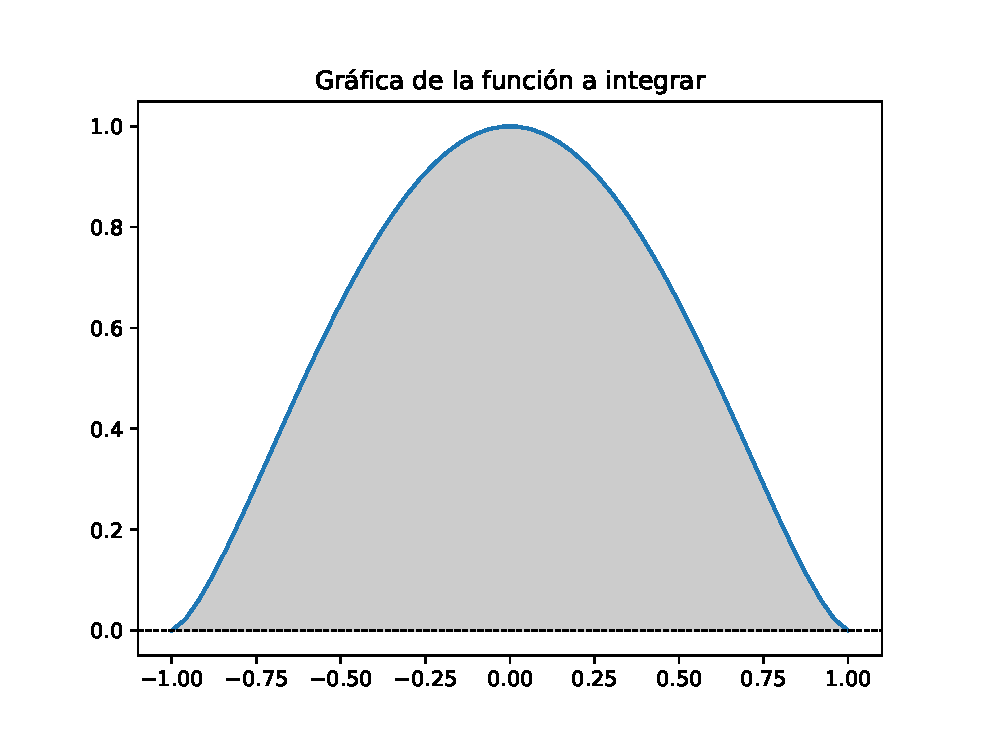
\includegraphics[scale=0.5]{Imagenes/cuadratura_01.eps}
	\caption{El área debajo de la curva, representa el valor de la integral.}
\end{figure}
\end{frame}
\end{document}

